\begin{figure}[h] 
\centering 
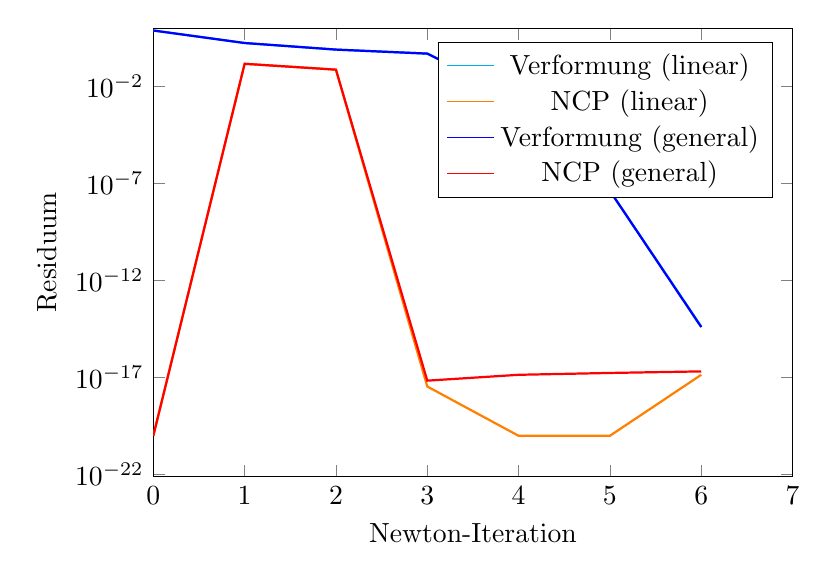
\begin{tikzpicture}[every plot/.append style={thick}] 
\begin{axis}[ 
label style={font=\normalsize}, 
xlabel={Newton-Iteration}, 
ylabel={Residuum}, 
xmin=0, xmax=7, 
ymode=log, 
ymin=0, ymax=10, 
width=0.8\textwidth, 
height=0.6\textwidth, 
legend pos=north east, 
legend style={cells={align=left}}, 
grid style=dashed, 
] 
\addplot[ 
color=cyan, 
] 
coordinates { 
(0, 7.64e+00)(1, 1.73e+00)(2, 7.93e-01)(3, 4.92e-01)(4, 2.39e-03)(5, 4.18e-08)(6, 4.29e-15)}; 
\addlegendentry{Verformung (linear)} 
\addplot[ 
color=orange, 
] 
coordinates { 
(0, 1.00e-20)(1, 1.47e-01)(2, 7.33e-02)(3, 3.47e-18)(4, 1.00e-20)(5, 1.00e-20)(6, 1.39e-17)}; 
\addlegendentry{NCP (linear)} 
\addplot[ 
color=blue, 
] 
coordinates { 
(0, 7.64e+00)(1, 1.73e+00)(2, 7.93e-01)(3, 4.92e-01)(4, 2.39e-03)(5, 4.18e-08)(6, 3.99e-15)}; 
\addlegendentry{Verformung (general)} 
\addplot[ 
color=red, 
] 
coordinates { 
(0, 1.00e-20)(1, 1.47e-01)(2, 7.33e-02)(3, 6.94e-18)(4, 1.39e-17)(5, 1.73e-17)(6, 2.08e-17)}; 
\addlegendentry{NCP (general)} 
\end{axis} 
\end{tikzpicture} 
\caption{Residuen des Stoffgesetzes 'Neo Hooke' mit Hinderniss 'Spitze' und 18 Freiheitsgraden für die Verschiebung.} 
\label{fiq:NeoHooke_Spitze_level0} 
\end{figure} 
